\documentclass[25pt]{article}
\usepackage[a4paper, top=3cm, left=3cm, right=2.5cm, bottom=2.5cm]{geometry}
\usepackage{lmodern}
\usepackage[T1]{fontenc}
\usepackage[portuges]{babel}
\usepackage[utf8]{inputenc}
\usepackage{a4}
\usepackage[document]{ragged2e}
\usepackage{textgreek}
\usepackage{epstopdf}
\usepackage{graphicx}
\usepackage{fancyvrb}
\usepackage{amsmath}
\usepackage{float}
\usepackage{listings}


\begin{document}

\begin{titlepage}

\newcommand{\HRule}{\rule{\linewidth}{0.5mm}} % Defines a new command for the horizontal lines, change thickness here

\center % Center everything on the page

%----------------------------------------------------------------------------------------
%	HEADING SECTIONS
%----------------------------------------------------------------------------------------

\textsc{\LARGE Universidade do Minho}\\[1.5cm]
\HRule \\[0.4cm]
{ \huge \bfseries Programação em Lógica e Invariantes}\\[0.4cm]
\HRule \\[1.5cm]
\textsc{\Large Mestrado Integrado em Engenharia Informática}\\[0.5cm]
\textsc{\large Sistemas de Representação de Conhecimento e Raciocínio}\\[0.5cm]
\textsc{\large 2ºSemestre 2018/19}\\[0.5cm]


%----------------------------------------------------------------------------------------
%	AUTHOR SECTION
%----------------------------------------------------------------------------------------

\begin{minipage}{0.4\textwidth}
\begin{flushleft} \large
\emph{Grupo:}\\
Etienne Costa A76089 \\
Joana Cruz A76270 \\
Rui Azevedo A80789 \\
Maurício Salgado A71407 \\
João Coutinho A86272 \\
\end{flushleft}
\end{minipage}
~
\begin{minipage}{0.4\textwidth}
\begin{flushright} \large
\emph{Docente:} \\
César Analide\\
\end{flushright}
\end{minipage}\\[2cm]

%----------------------------------------------------------------------------------------
%	DATE SECTION
%----------------------------------------------------------------------------------------

{\large \today}\\[2cm]

%----------------------------------------------------------------------------------------
%	LOGO SECTION
%----------------------------------------------------------------------------------------

% 
\includegraphics[scale=0.3]{uminho}\\

%----------------------------------------------------------------------------------------

\vfill % Fill the rest of the page with whitespace

\end{titlepage}
\section{Resumo}
 O presente trabalho tem como principal objetivo aprofundar os conhecimentos na linguagem de programação em lógica PROLOG.\newline
 Com base nisso foi desenvolvido o relatório explicando o desenvolvimento do primeiro exercício prático no âmbito da unidade
 curricular de Sistemas de Representação de Conhecimento e Raciocínio.\newline
 Este trabalho desenvolvido consiste na implementação de um sistema de representação de conhecimento e raciocínio com capacidade
 para caracterizar um universo de discurso na área da prestação de cuidados de saúde.\newline



\newpage
\tableofcontents
\newpage
\section{Introdução}
O relatório apresentado diz respeito ao primeiro exercício proposto no âmbito da unidade curricular de Sistemas de
Conhecimento de Representação e Raciocínio, utilizando a linguagem de programação em lógica PROLOG. O universo de discurso
para qual estamos a desenvolver este sistema é o universo de prestação de cuidados de saúde, assim esta base de conhecimento consiste
em utentes, serviços, consultas, prestadores de serviços, medicamentos e receitas.
\newpage
\section{Preliminares}
Para o desenvolvimento deste projeto foi necessário alguns conhecimentos previamente adquiridos de programação em lógica, e a
utilização da linguagem PROLOG. Este conhecimento foi absorvido durante as aulas de Sistemas de Representação de Conhecimento e Raciocínio,
e também com alguma pesquisa nossa. De seguida, apresentamos alguns conceitos fundamentais para a compreensão e realização deste trabalho.
\subsection{Programação em lógica e PROLOG}
Uma das principais ideias da programação em lógica é de que um algoritmo é constituído por dois
elementos disjuntos: a lógica e o controle. O componente lógico corresponde à definição do que deve
ser solucionado, enquanto que o componente de controle estabelece como a solução pode ser obtida.
O programador precisa somente descrever o componente lógico de um algoritmo, deixando o controle
da execução para ser exercido pelo sistema de programação em lógica utilizado. Em outras palavras, a
tarefa do programador passa a ser simplesmente a especificação do problema que deve ser solucionado, razão pela qual as
linguagens lógicas podem ser vistas simultaneamente como linguagens para
especificação formal e linguagens para a programação de computadores.
O paradigma fundamental da programação em lógica é o da programação declarativa, em oposição à
programação procedimental típica das linguagens convencionais.
Um programa em lógica é então a representação de determinado problema ou situação expressa através de um conjunto finito
de um tipo especial de sentenças lógicas denominadas cláusulas.
Pode-se então expressar conhecimento (programas e/ou dados) em Prolog por meio de cláusulas de
dois tipos: fatos e regras. Um fato denota uma verdade incondicional, enquanto que as regras definem as condições que devem ser satisfeitas para que
uma certa declaração seja considerada verdadeira. Como fatos e regras podem ser utilizados conjuntamente, nenhum componente
dedutivo adicional precisa ser utilizado. Além disso, como regras recursivas e não-determinismo são permitidos, os programadores podem obter
descrições muito claras, concisas e não-redundantes da informação que desejam representar. Como não há distinção entre argumentos
de entrada e de saída, qualquer combinação de argumentos pode ser empregada.
Os termos "programação em lógica" e "programação Prolog" tendem a ser empregados indistintamente. Deve-se, entretanto, destacar
que a linguagem Prolog é apenas uma particular abordagem da
programação em lógica.
\newpage
\section{Base de conhecimento}
Um programa em Prolog é um conjunto de axiomas e de regras de inferência definindo relações entre objectos que descrevem
um dado problema. A este conjunto chama-se normalmente base de conhecimento.\\
A base de conhecimento do sistema desenvolvido é essencial à representação do conhecimento e raciocínio,tendo em conta o sistema
foram desenvolvidas as seguintes entidades:

\begin{itemize}
  \item utente: \#IdUt, Nome, Idade,Sexo, Cidade $\to$ \{V,F\}
  \item serviço: \#IdServ,Especialidade,Instituiç\~ao,Cidade $\to$ \{V,F\}
  \item consulta:\#IdConsult,\#IdUt,\#IdPrestador,\#IdServ,Descrição,Custo,Data $\to$ \{V,F\}
  \item prestador:\#IdPrestador,\#IdServ,Nome,Idade,Sexo $\to$ \{V,F\}
  \item medicamento:\#IdMed,Nome,Custo $\to$ \{V,F\}
  \item receita:\#IdCons,\#IdMed,DataValidade,Quantidade $\to$ \{V,F\}
  \end{itemize}



\subsection{Análise conceptual do problema}
Depois de uma análise ao contexto do problema, foi elaborado um esquema conceptual do mesmo. Dado o enunciado conseguimos identificar as
seguintes entidades Utente, Serviço e Consulta. De forma a garantir uma melhor consistência da nossa Base de Conhecimento utilizamos a entidade Prestador de Serviço, e a aumentar
este sistema cujo universo é o de prestação de cuidados de saúde identificamos as entidades Receita e Medicamento.
\begin{figure}[H]
\centering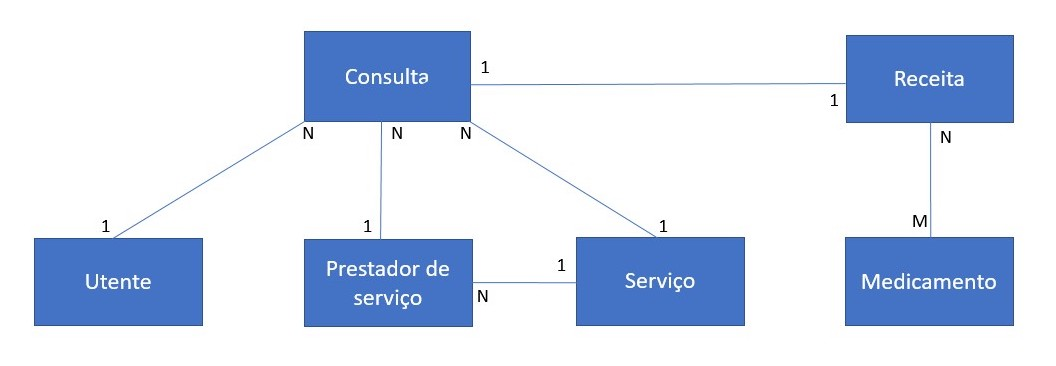
\includegraphics[scale=0.35]{esquema}
\caption{\label{fig:controller}Esquema conceptual representativo do problema}
\end{figure}
Tentamos abordar este problema o mais perto de contextos reais, sendo que em todos os hospitais e clinicas existem consultas, que são sempre
referentes a um utente, um prestador de serviço e a um serviço.
\subsection{Entidades}
Nesta secção são apresentadas e caraterizadas as Entidades acima propostas.

\subsubsection{Utente}
Num mundo real o utente é caracterizado por diversos factores , que por sua vez no contexto do Prolog esses factores passam a ser denomindados por átomos cujo o seu propósito é identifcar os objectos. Sendo assim para os utentes optou-se por usar os seguintes átomos:


 \begin{itemize}
  \item IdUt: Identificador do utente,que por sua vez é um valor único.
  \item Nome: Nome do utente.
  \item Idade: Idade do utente.
  \item Sexo: Sexo do utente.
  \item Cidade: Cidade aonde mora o utente.
\end{itemize}

\subsubsection{Serviço}
Um serviço por sua vez é  caracterizado pelos seguintes átomos:
\begin{itemize}
  \item IdServ: Identificador do serviço, que por sua vez é uma valor único.
  \item Especialidade: Referente ao serviço prestado.
  \item Instituição: Espaço físico aonde é efectuado o serviço.
  \item Cidade: Espaço geográfico aonde se encontra a instituição.
\end{itemize}

\subsubsection{Consulta}
Uma consulta será sempre referente a um utente, a um prestador de serviço e a um serviço, sendo que a mesma é realizada numa data específica e tem sempre uma breve descrição e custo associado , portanto optou-se por representar o conhecimento do seguinte modo:

\begin{itemize}
  \item IdConsult: Identificador da consulta, que por sua vez é uma valor único.
  \item IdUt: Identificador do utente.
  \item IdPrestador: Identificador do prestador de serviço.
  \item IdServ: Identificador do serviço prestado.
  \item Descrição:Breve descrição da consulta.
  \item Custo: Custo associado à consulta.
  \item Data: Data da realização da consulta.
\end{itemize}

\subsubsection{Prestador}
O prestador por sua vez é a entidade que presta os serviços existentes na base de conhecimento e para tal o mesmo é caracterizado pelos seguintes
átomos:

\begin{itemize}
  \item IdPrestador: Identificador do prestador, que por sua vez é uma valor único.
  \item IdServ: Identificador do serviço prestado.
  \item Nome:   Nome do prestador de serviço.
  \item Idade:  Idade do prestador.
  \item Sexo:   Sexo do prestador.
 \end{itemize}


\subsubsection{Medicamento}
Sendo que estamos presente a um sistema de prestação de cuidados de saúde,sentimo-nos na obrigação de fazer a inserção dos medicamentos na base
de conhecimento visto que na maioria das vezes após o término de uma consulta é passada uma receita que é constituída por diversos medicamentos.
Com base nisso os medicamentos são caracterizados por :

\begin{itemize}
  \item IdMed: Identificador do medicamento, que por sua vez é uma valor único.
  \item Nome: Nome do medicamento.
  \item Custo:  Custo do medicamento.
 \end{itemize}



\subsubsection{Receita}
A receita é uma rotina de cuidados com a saúde, implementadas pelo prestador, voltadas para um utente em específico. Sendo assim a receita é caracterizada por :

\begin{itemize}
  \item IdCons: Identificador da consulta, que por sua vez é uma valor único.
  \item IdMed: Identificador do medicamento.
  \item DataValidade:  Corresponde a data de validade de uma receita.
  \item Quantidade: Corresponde a quantidade de um medicamento pertencente à receita.
 \end{itemize}

\newpage

\section{Integridade da Base de Conhecimento}
De forma a manter a integridade da base do conhecimento, e esta esteja de acordo com a realidade que pretendemos representar,é necessário implementar
algum mecanismo que nos garanta isso. Assim, ao longo do trabalho fomos dando uso ao conceito de invariante. Estes permitem-nos controlar em específico a
correta inserção e remoção na Base de Conhecimento. Os invariantes em PROLOG são representados da seguinte forma:
\begin{itemize}
\item +Termo :: Premissas.
\item -Termo :: Premissas.
\end{itemize}
Em Prolog, já existem predicados que nos permitem inserir e remover factos da Base de Conhecimento. Estes são o assert e o retract, respetivamente. No entanto, a utilização destes predicados, exclusivamente, não garante consistência. Sendo assim, é necessário a criação de predicados auxiliares que nos garantam a intregidade da Base de Conhecimento.

\subsection{Inserção de Conhecimento}
Como já havia sido dito anteriormente o uso exclusivo da função assert não garante a integridade, para tal surgiu um conjunto de condições que são
verificadas de modo a presevar a consistência da base de conhecimento, e só assim inserir conhecimento. Este processo foi denominado por evolução.
É Implementado do seguinte modo:
\begin{lstlisting}
evolucao(T) :-
findall( I,+T::I,Li ),
insercao( T ),
teste( Li ).

insercao(T) :- assert(T).
insercao(T) :- retract(T), !, fail.
\end{lstlisting}

\subsection{Remoção de conhecimento}

Para a remoção do conhecimento o processo foi análogo ao de inserção, só que para este caso concreto o uso exclusivo do retract não garante a integridade, para tal surgiu um conjunto de condições de modo a preservar a consistência da base de conhecimento, e só assim remover conhecimento.
Este processo foi denominado por involução.É implementado do seguinte modo:

\begin{lstlisting}
involucao(T) :- T,
findall(I,-T::I,Li),
remocao(T),
teste(Li).

remocao(T) :- retract(T).
remocao(T) :- assert(T), !, fail.
\end{lstlisting}

\subsection{Invariantes Estruturais}
Os invariantes estruturais são, tal como o nome indica, responsáveis por manter a estrutura do conhecimento existente. Foi
necessário garantir que as inserções não pudessem introduzir conhecimento repetido e que as remoções não pudessem retirar
conhecimento não existente ou que estaria associado a outros.

\subsubsection{Invariantes de inserção}
Este processo é implementado de forma similar em todos os casos referentes aos invariantes de inserção.\newline



Este invariante permite garantir que o identificador de cada utente é  único e do tipo inteiro.

\begin{lstlisting}
  +utente(IdUt,_,_,_,_) ::
  (integer(IdUt),
  findall(IdUt,utente(IdUt,Nome,Idade,Sexo,Cidade),S),
  length(S,L),
  L == 1).
\end{lstlisting}


Este invariante permite garantir que o identificador de cada serviço é  único e do tipo inteiro.\\

\begin{lstlisting}
+servico(IdServ,_,_,_) ::
(integer(IdServ),
findall(IdServ,servico(IdServ,_,_,_),S),
length(S,L),L == 1).
\end{lstlisting}

Sendo que a consulta envolve as diferentes chaves primárias da nossa base de conhecimento, houve o cuidado de garantir que o Idconsult é único e do tipo inteiro,e não só,para ser registada uma consulta faz sentido garantir que existe pelo  a ocorrência do respectivo utente,prestador e o serviço prestado,sendo esses representados no invariante  através dos respectivos identificadores.\\
\begin{lstlisting}
 +consulta(IdConsult,IdUt,IdPrestador,IdServ,_,_,_)::
 (integer(IdConsult),
 utente(IdUt,_,_,_,_),
 prestador(IdPrestador,IdServ,_,_,_),
 servico(IdServ,_,_,_),
 findall(IdConsult,consulta(IdConsult,_,_,_,_,_,_),S),
 length(S,N),
 N==1).
\end{lstlisting}


O invariante de inserção do prestador segue a mesma lógica que o invariante do utente, sendo que este tem um caso particular que corresponde ao serviço na qual é especializado,ou seja, para efectuar a inserção de um prestador o serviço no qual é especializado  deve existir.\\
\begin{lstlisting}
  +prestador(IdPrest,IdServ,_,_,_) ::
  (integer(IdPrest),
  servico(IdServ,_,_,_),
  findall(IdPrest,prestador(IdPrest,_,_,_,_),S),
  length(S,L) , L== 1).
\end{lstlisting}



Este invariante permite garantir que o identificador de cada medicamento é  único e do tipo inteiro.\\
\begin{lstlisting}

+medicamento(IdMed,_,_) ::
(integer(IdMed),
findall(IdMed,medicamento(IdMed,_,_),S),
length(S,L) , L == 1).
\end{lstlisting}


Relativamente a receita usa-se a combinação de dois identificadores para verificar se ocorreu a respectiva consulta e o identificar do medicamento
para confirmar que o mesmo existe na base de conhecimento.
\begin{lstlisting}
+receita(IdCons,IdMed,_,_) ::
(integer(IdCons) ,
integer(IdMed),
consulta(IdCons,_,_,_,_,_,_),
medicamento(IdMed,_,_),
findall((IdCons,IdMed),receita(IdCons,IdMed,_,_),S),
length(S,L) , L == 1).
\end{lstlisting}




\subsubsection{Invariantes de remoção}

Quanto aos invariantes de remoção  seguem todos a mesma ideologia,sendo que só faz sentido fazer uma remoção da base de conhecimento de algo existente na mesma.

\begin{lstlisting}
-utente(IdUt,_,_,_,_) ::
(findall(IdUt,utente(IdUt,_,_,_,_),S),
length(S,N),
N==0).
\end{lstlisting}

\begin{lstlisting}
-servico(IdServ,_,_,_) ::
(findall(IdServ,servico(IdServ,_,_,_),S),
length(S,N),
N==0).
\end{lstlisting}

\begin{lstlisting}
-prestador(IdPrest,_,_,_,_,_) ::
(integer(IdPrest),
findall(IdPrest,prestador(IdPrest,_,_,_,_,_),S),
length(S,L),
L == 0).
\end{lstlisting}

\begin{lstlisting}
-medicamento(IdMed,_,_) ::
(integer(IdMed),
findall(IdMed,medicamento(IdMed,_,_),S),
length(S,L),
L == 0).
\end{lstlisting}




\subsection{Invariantes Referenciais}
Os invariantes referenciais evitam que as regras lógicas associadas ao domínio
de conhecimento sejam quebradas, permitindo manter a integridade dos dados.\newpage

Relativamente ao utente e o prestador foi necessário garantir que a idade dos mesmos fosse maior ou igual que zero e que o sexo  seja  'M' ou 'F',sendo que para a  validação do sexo foi utilizado um predicado auxiliar validaSexo.\\

\begin{lstlisting}
+utente(_,_,Idade,Sexo,_) ::
(integer(Idade),
Idade >= 0,
validaSexo(Sexo)).
\end{lstlisting}


\begin{lstlisting}
+prestador(_,_,_,Idade,Sexo) ::
(integer(Idade),
Idade >=0,
validaSexo(Sexo)).
\end{lstlisting}


No que concerne a consulta foi importante garantir  que o seu custo é superior ou igual à 0 u.m e que a sua data seja válida tirando partido do predicado auxilar validaData.
\begin{lstlisting}

 +consulta(_,_,_,_,_,Custo,Data) ::
 (validaData(Data),
 Custo>=0).
\end{lstlisting}



Quanto aos medicamentos tivemos que garantir que o seu custo fosse sempre superior à 0 u.m.
\begin{lstlisting}
+medicamento(_,_,Custo) ::
(Custo > 0).
\end{lstlisting}


Relativamente a receita procuramos inserir uma data de modo a enquadar-se num contexto real , visto que as mesmas possuem um prazo e para tal
essa data deve ser válida, e a quantidade de cada medicamento receitada não pode ser superior à 5 unidades
\begin{lstlisting}
+receita(_,_,DataValidade,Quantidade) ::
(validaData(DataValidade),
Quantidade > 0).
\end{lstlisting}


\newpage
\section{Funcionalidades}

\subsection{Registar utentes,serviços,consultas,prestadores,medicamentos e receitas}
\begin{figure}[H]
\centering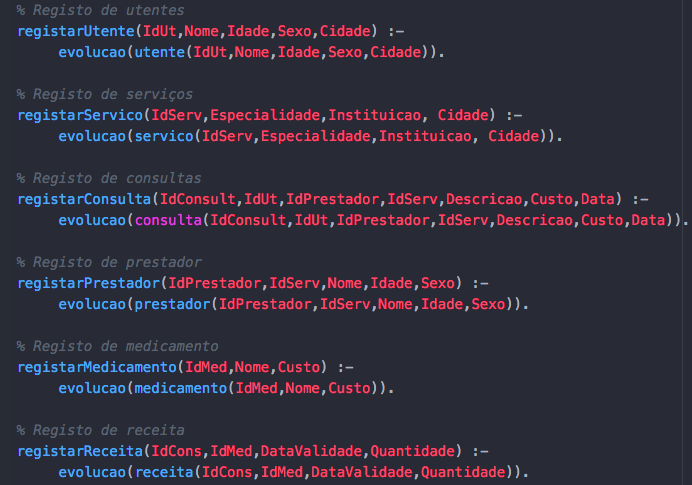
\includegraphics[scale=0.5]{registo}
\caption{\label{fig:controller}Registo dos principais intervenientes do sistema}
\end{figure}


\subsection{Remover utentes,serviços,consultas,prestadores,medicamentos e receitas}
\begin{figure}[H]
\centering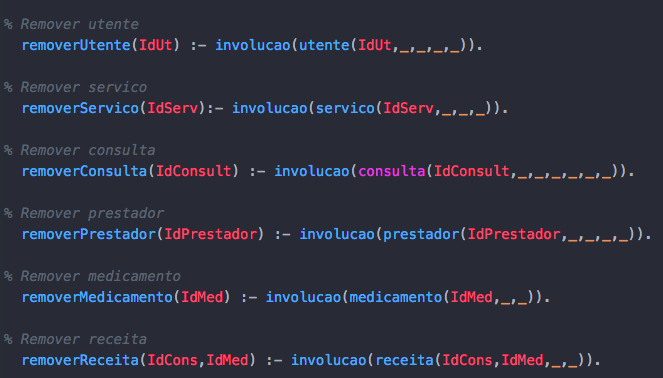
\includegraphics[scale=0.5]{Remocoes}
\caption{\label{fig:controller}Remocão dos principais intervenientes do sistema}
\end{figure}


\subsection{Identificação das instituições prestadoras de serviços}

\begin{figure}[H]
\centering
\includegraphics[scale=0.7]{listarI}
\caption{\label{fig:controller}Listar Instituições}
\end{figure}

\subsection{Identificação de utentes por critérios de seleção}
\begin{figure}[H]
\centering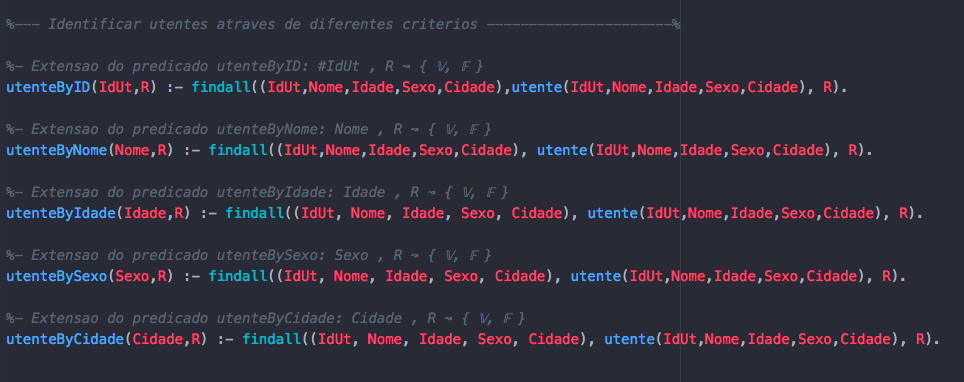
\includegraphics[scale=0.5]{criterioutente}
\caption{\label{fig:controller}Identificação de utentes}
\end{figure}

\subsection{Identificação de prestadores por critérios de seleção}
\begin{figure}[H]
\centering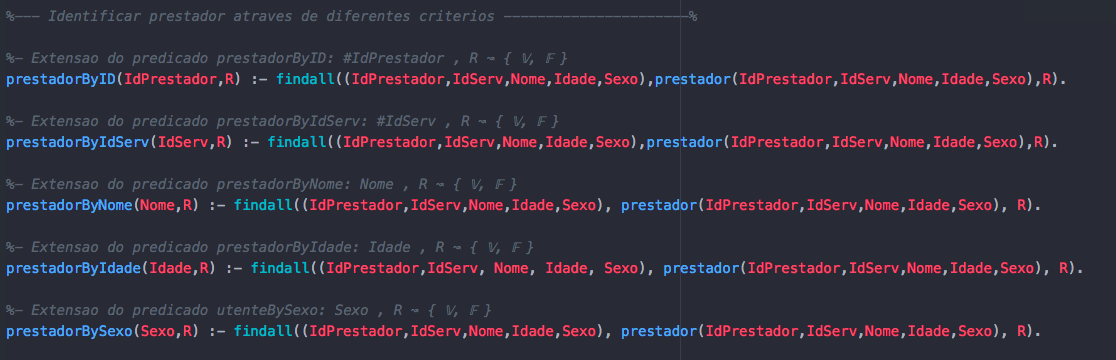
\includegraphics[scale=0.45]{prestador}
\caption{\label{fig:controller}Identificação de prestadores}
\end{figure}

\subsection{Identificação de medicamentos por critérios de seleção}
\begin{figure}[H]
\centering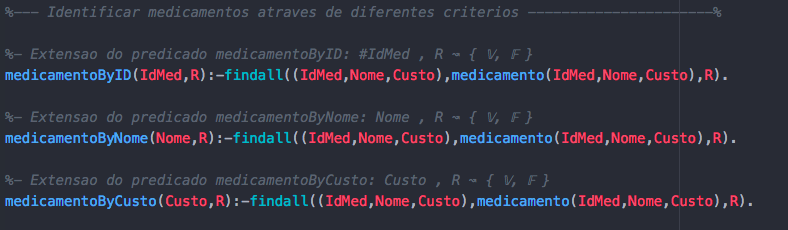
\includegraphics[scale=0.5]{medicamento}
\caption{\label{fig:controller}Identificação de medicamentos}
\end{figure}


\subsection{Identificação de receitas por critérios de seleção}
\begin{figure}[H]
\centering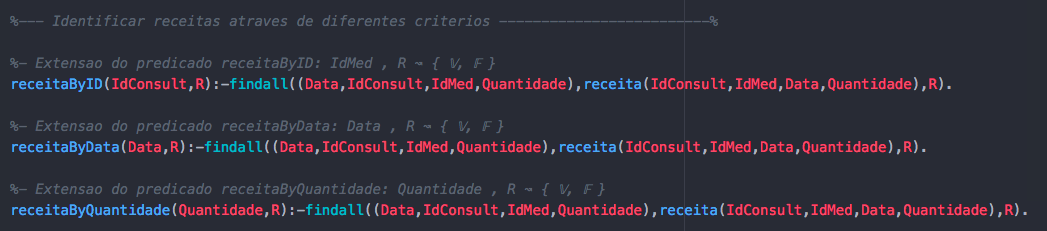
\includegraphics[scale=0.45]{receita}
\caption{\label{fig:controller}Identificação de receitas}
\end{figure}
\subsection{Identificação de serviços por critérios de seleção}
\begin{figure}[H]
\centering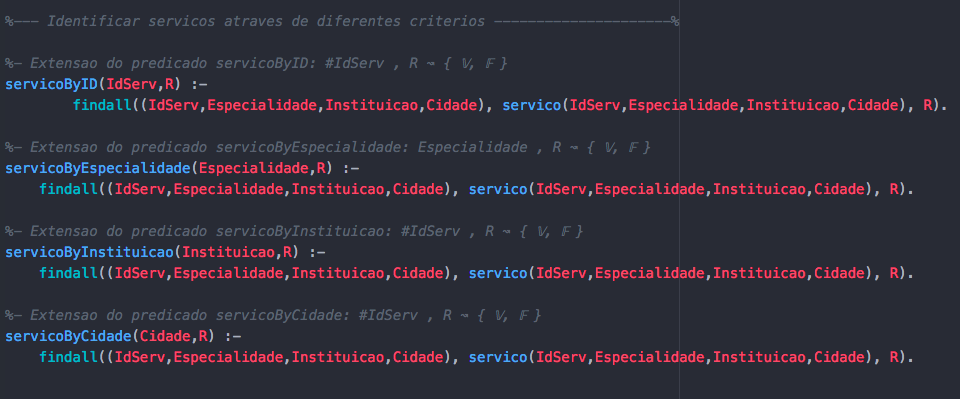
\includegraphics[scale=0.5]{criterioservico}
\caption{\label{fig:controller}Identificação de serviços}
\end{figure}
\subsection{Identificação de consultas por critérios de seleção}
\begin{figure}[H]
\centering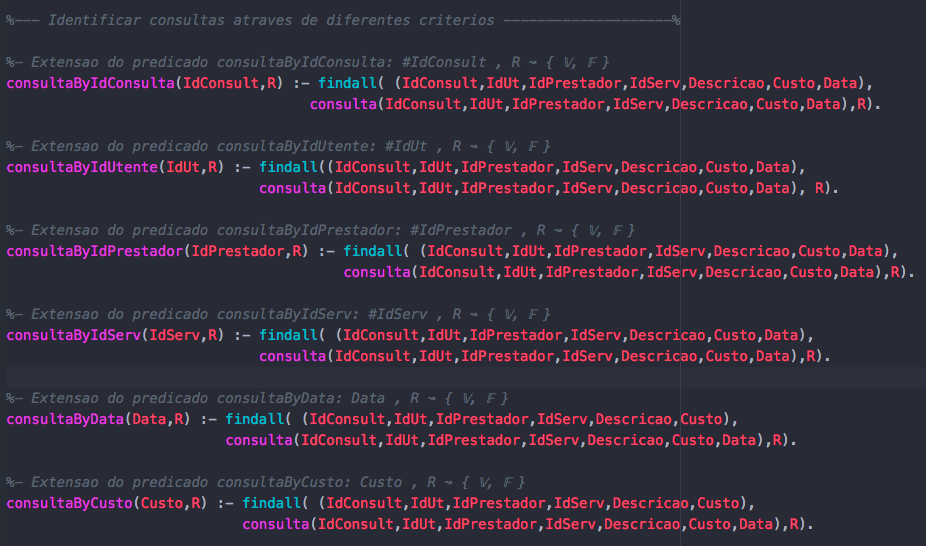
\includegraphics[scale=0.5]{criterioconsulta}
\caption{\label{fig:controller}Identificação de consultas}
\end{figure}
\subsection{Identificação de serviços prestados por instituição/cidade}
\begin{figure}[H]
\centering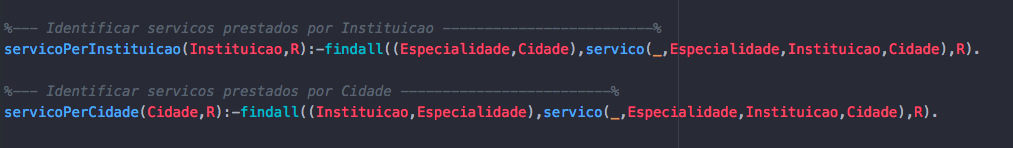
\includegraphics[scale=0.5]{PerInsCidade}
\caption{\label{fig:controller}Identificação de serviços por instituição e cidade}
\end{figure}

\subsection{Identificação de utentes de um serviço/instituição}

\begin{figure}[H]
\centering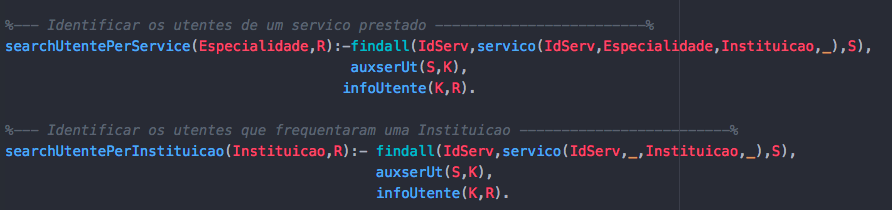
\includegraphics[scale=0.5]{Perserviceinst}
\caption{\label{fig:controller}Identificação de utentes que frequentaram um serviço ou instituição}
\end{figure}

\subsection{Identificação de serviços realizados por utente/instituição/data/custo}
\begin{figure}[H]
\centering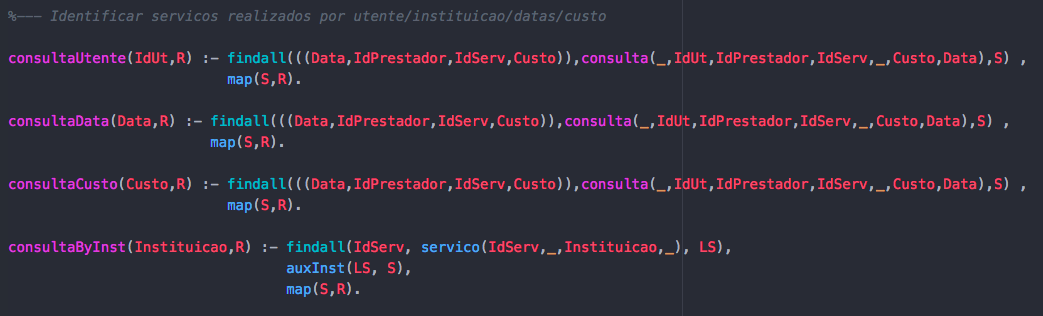
\includegraphics[scale=0.45]{consulta}
\caption{\label{fig:controller}Consultas concretizadas }
\end{figure}

\subsection{Cálculo do custo total dos cuidados de saúde por utente/serviço/instituição/data}


\begin{figure}[H]
\centering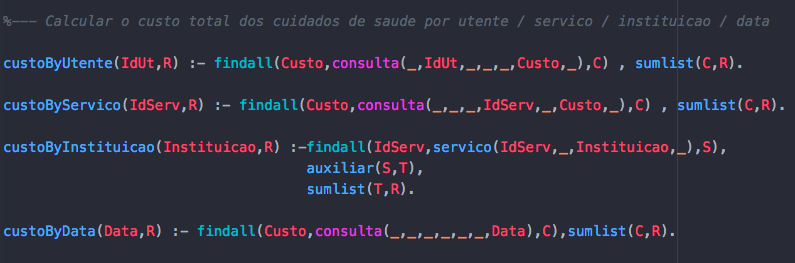
\includegraphics[scale=0.5]{custo}
\caption{\label{fig:controller}Custos}
\end{figure}
\newpage

\section{Extras}
De forma voluntária decidimos acrescentar novas funcionalidades de acordo com a nossa base de conhecimento,isto é, invariantes referenciais e estruturais sobre os predicados prestador,receita e medicamentos estando os mesmos referenciados acima.
De forma a explorar informação sobre os mesmos foram implementadas as seguintes funcionalidades:


\begin{itemize}
  \item getCustoReceita : Devolve o custo total de uma receita.
  \begin{lstlisting}
  getCustoReceita(IdCons, R) :-
  findall((IdMed,Quantidade),receita(IdCons,IdMed,_,Quantidade),S),
  getCustoMedicamento(S,R).
  \end{lstlisting}

  \item getPrestadores : Dado o identificador de um utente, retorna a lista dos prestadores de serviços que o utente frequentou e as suas respectivas datas.
  \begin{lstlisting}
  getPrestadores(IdUt , R) :-
  findall((IdPrest,Data),consulta(_,IdUt,IdPrest,_,_,_,Data),S1) ,
  auxiliarPrestador(S1,R).
  \end{lstlisting}

  \item getMedicamentosByReceita: Dado o identificador da consulta, lista os medicamentos que fazem parte desta receita.
  \begin{lstlisting}
  getMedicamentosByReceita(IdConsult, R) :-
  findall(IdMed,receita(IdConsult, IdMed,_,_), S),
  auxiliarMedicamentos(S,R).
  \end{lstlisting}

  \item getNumeroMedicosByInst: Devolve o número de prestadores de uma dada especialidade em uma dada instiuição.
  \begin{lstlisting}
  getNumeroMedicosByInst(Especialidade, Instituicao, R) :-
  findall(IdServ,servico(IdServ,Especialidade,Instituicao,_),S1) ,
  head(S1,H),
  findall(IdPrest,prestador(IdPrest,H,_,_,_), S2),
  length(S2,R).
  \end{lstlisting}


 \item despesaAnualConsultas: Devolve o total gasto por um utente em um determinado ano.
 \begin{lstlisting}
 despesaAnualConsultas(IdUt, Ano, R) :-
 findall(Custo,consulta(_,IdUt,_,_,_,Custo,(Ano,_,_)), S),
 sumlist(S,R).
 \end{lstlisting}

 \item medicamentoMaisCaro : Devolve o medicamento mais caro.
 \begin{lstlisting}
 medicamentoMaisCaro(R) :-
 findall((Custo,Nome), medicamento(_,Nome,Custo),S) ,
 sort(S,N) ,
 last(N,L),
 swap_pair(L,R).
\end{lstlisting}

 \item medicamentoMaisBarato : Devolve o medicamento mais barato.

 \begin{lstlisting}
 medicamentoMaisBarato(R) :-
 findall((Custo, Nome), medicamento(_,Nome,Custo),S),
 sort(S,N),
 head(N,L),
 swap_pair(L,R).
\end{lstlisting}


\item freq\_esp: Dada uma especialidade devolve a frequencia de utentes dessa
especialidade.

\begin{lstlisting}
freq_esp(Especialidade, R) :-
findall(IdServ, servico(IdServ,Especialidade,_,_), L),
auxFreq(L, S),
findall(IdConsult, consulta(IdConsult,_,_,_,_,_,_), A),
length(S,S1), length(A,A1),
R is S1/A1 * 100.
\end{lstlisting}


\item freq\_all: Devolve as frequencias de utentes de todas as especialidades.
\begin{lstlisting}
freq_all(R) :-
findall(Especialidade, servico(_,Especialidade,_,_), L),
sort(L, L1),
maplist(freq_esp, L1, L2),
zip(L1, L2, R).
\end{lstlisting}

 \end{itemize}

 Além destas funcionalidades inserimos ainda um Menu, de modo que futuros utilizadores possam tirar partido do sistema desenvolvido
 sem perceber concretamente como o mesma está implementado.


 \begin{figure}[H]
 \centering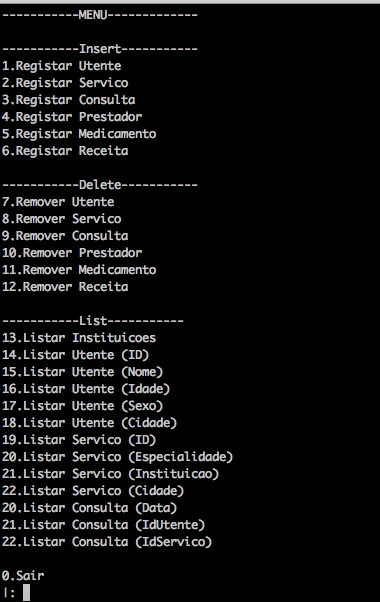
\includegraphics[scale=0.45]{menu}
 \caption{\label{fig:controller}Esquema conceptual representativo do problema}
 \end{figure}
\newpage

\section{Conclusão}
A realização deste trabalho prático permitiu consolidar o conhecimento adquirido ao longo das aulas, no que concerne
à programação em lógica e invariantes. Como tal, o suporte utilizado para caracterizar um universo de discurso na área da prestação de cuidados de
saúde foi o PROLOG.
Para o sistema em causa procurou-se fazer sempre uma aproximação ao contexto real do problema sendo que toda  base de conhecimento surge à custa de um
modelo conceptual, procurando não repetir conhecimento e inserir funcionalidades extras de modo a representar o conhecimento de forma inteligente.
Em forma de conclusão, podemos afirmar que fomos capazes de aplicar os conhecimentos lecionados e com êxito implementar as funcionalidades exigidas , sendo que de forma voluntária foram implementadas algumas funcionalidades extras.
\newpage
\section{Referências Bibliográficas}


\newpage

\section{Funções Auxiliares}
\begin{lstlisting}
%----------------------------------------------------------------------------------------
auxiliar([],[]).
auxiliar([IdServ|Tail],R):-
findall(Custo,consulta(_,_,_,IdServ,_,Custo,_),S),
auxiliar(Tail,T),
append(S,T,R).
%----------------------------------------------------------------------------------------
auxiliarPrestador([],[]).
auxiliarPrestador([(IdPrest,Ano,Mes,Dia)|Tail],R) :-
findall(Nome,prestador(IdPrest,_,Nome,_,_,_),S),
auxiliarPrestador(Tail,T),
head(S,P) ,
append([P,Ano,Mes,Dia],T,R).
%----------------------------------------------------------------------------------------
auxiliarMedicamentos([],[]).
auxiliarMedicamentos([IdMed|Tail],R) :-
findall(Nome,medicamento(IdMed,Nome,_),S),
auxiliarMedicamentos(Tail,T),
append(S,T,R).
%----------------------------------------------------------------------------------------
auxInst([],[]).
auxInst([IdServ|Tail], R) :-
findall((Data,IdPrestador,IdServ,Custo),
consulta(_,_,IdPrestador,IdServ,_,Custo,Data), L),
auxInst(Tail,S),
append(L,S,R).
%----------------------------------------------------------------------------------------
map([],[]).
map([((Data,IdPrestador,IdServ,Custo))|Tail],R) :-
map(Tail,T) ,
findall(Nome,prestador(IdPrestador,_,Nome,_,_),P) ,
findall(Especialidade,servico(IdServ,Especialidade,_,_),S),
findall(Instituicao,servico(IdServ,_,Instituicao,_),Q),
head(P,PR) , head(S,SR) ,head(Q,INS),
append([(Data,PR,SR,Custo,INS)],T,R).
%----------------------------------------------------------------------------------------
zip([],[],[]).
zip([X|XS],[Y|YS], [(X,Y)|Z]) :- zip(XS,YS,Z).

%----------------------------------------------------------------------------------------
infoUtente([],[]).
infoUtente([IdUt|Tail],R):-findall((IdUt,Nome,Idade,Sexo,Cidade),
utente(IdUt,Nome,Idade,Sexo,Cidade),S),
infoUtente(Tail,T),
append(S,T,R).
%----------------------------------------------------------------------------------------
auxserUt([],[]).
auxserUt([Id|Tail],R):-
findall(IdUt,consulta(_,IdUt,_,Id,_,_,_),S),
auxserUt(Tail,T),
append(S,T,K),
sort(K,R).
%----------------------------------------------------------------------------------------
getCustoMedicamento([],0).
getCustoMedicamento([Head | Tail] , R) :-
getCustoMedicamento(Tail,S1),
factor(Head,S2),
R is S1 + S2.
%----------------------------------------------------------------------------------------
factor((IdMed,Quantidade), R) :-
findall(Custo, medicamento(IdMed,_,Custo), S) ,
head(S,S1) ,
R is S1 * Quantidade.

%----------------------------------------------------------------------------------------

auxFreq([],[]).
auxFreq([IdServ|Tail], R) :-
findall(IdConsult, consulta(IdConsult,_,_,IdServ,_,_,_), L),
auxFreq(Tail, S),
append(L,S,R).
%----------------------------------------------------------------------------------------

swap_pair((X,Y),(Y,X)).
%----------------------------------------------------------------------------------------

\end{lstlisting}
\end{document}
